\chapter{Review of Heavy Flavor Results}

In the previous section, we have introduced the relativistic heavy-ion physics and heavy flavor physics in vacuum and QGP. Physicists propose many experimental observables to study open heavy flavor physics and test theoretical models in heavy ion collisions. Traditionally, heavy flavor hadron $v_2$, $R_{AA}$, and production yield ratio are extensively studied. In this section, we will review selected experimental and theoretical results results in this section and discuss the physics messages from the measurements.


\section{Elliptic Flow}


In the QGP medium, heavy quarks are diffused by the color force and multiple scatter with medium constituents, which could generate sizable azimuthal anisotropy $v_2$ \cite{HQReview}. In addition, due to the azimuthal anisotropic expansion of the medium, the different path lengths of heavy quarks are different in different direction, which will also contribute to . Experimentally, we scale the $v_2$ and the hadron kinetic energy $K_T = \sqrt{m^2 + p_T^2} - m^2$ of heavy quarks with $n_q$ according to the Number of Constituent Quark (NCQ) Scaling in quark coalescence model \cite{NCDScaling}. Figure \ref{HQV2} shows the comparison of the $v_2/n_q$ as a function of $K_T/n_q$ of $D^0$ ($c\bar u$) meson with light flavor hadrons with STAR experiments at RHIC \cite{STARD0v2} and the CMS experiment at LHC \cite{CMSD0v2}.


\begin{figure}[hbtp]
\begin{center}
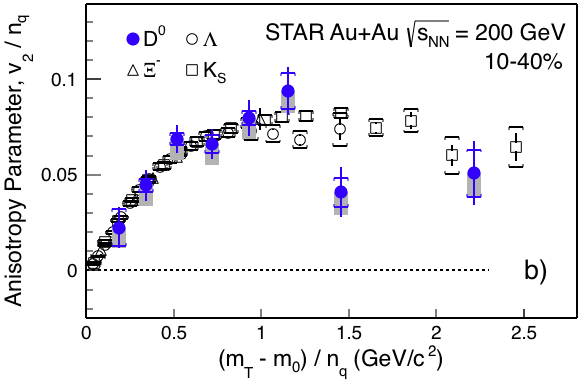
\includegraphics[width=0.50\textwidth]{Figures/Chapter2/STARv2.png}
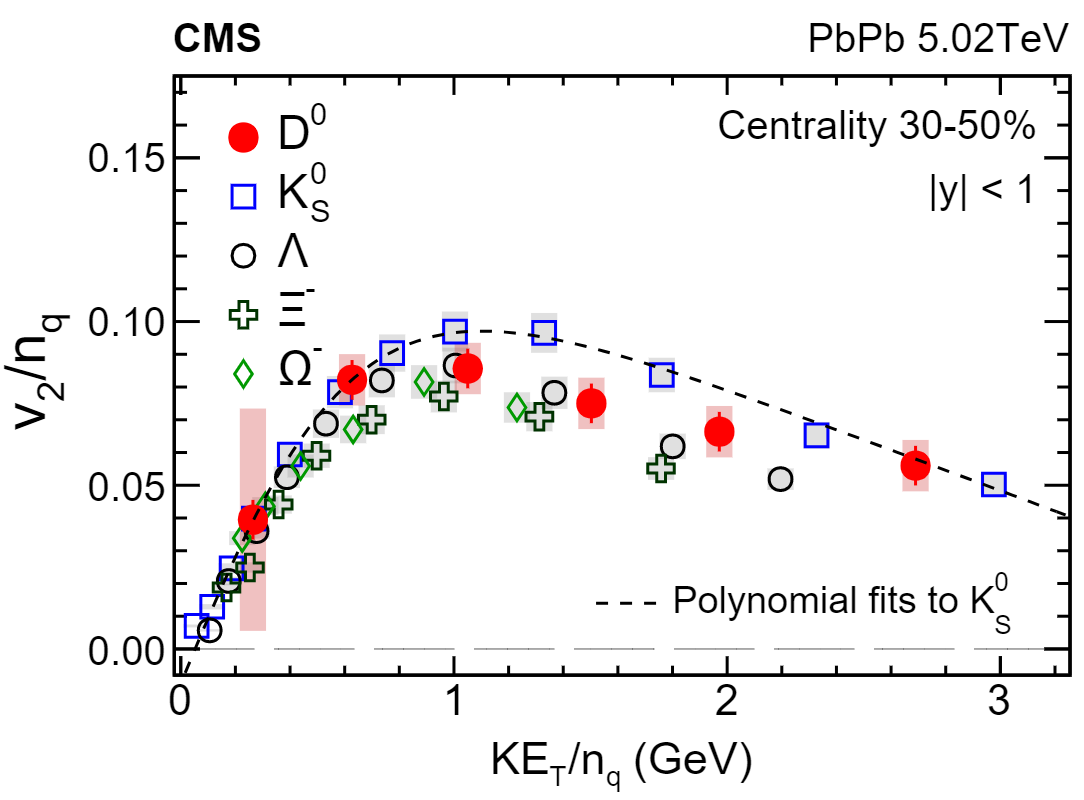
\includegraphics[width=0.485\textwidth]{Figures/Chapter2/CMSv2.png}
\caption{The NCQ scaled $D^0$ $v2/n_q$ vs $K_T/n_q$ and the comparison light hardons measured by the STAR experiment at RHIC (left) and the CMS experiment at LHC (right) are shown above.}
\label{HQV2}
\end{center}
\end{figure}   

We could see a reasonably good NCQ scaling behavior of $D^0$ meson with other light flavor hadrons, which suggests sizable collectivity of charm quarks in the QGP medium. To study azimuthal anisotropy of beauty quarks, an indirect approach is employed. Figure \ref{BeautyEV2} shows the elliptic flow of electron from beauty hadrons $b (\rightarrow c) \rightarrow e$ measured by the ALICE experiment \cite{ALICENPElec} and muon from beauty hadrons $b \rightarrow \mu$ measured by the ATLAS experiment \cite{ATLASNPMuon}


\begin{figure}[hbtp]
\begin{center}
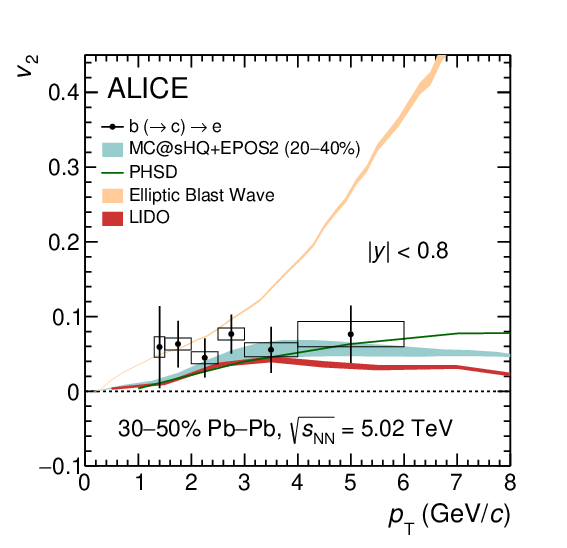
\includegraphics[width=0.50\textwidth]{Figures/Chapter2/ALICENPEv2.png}
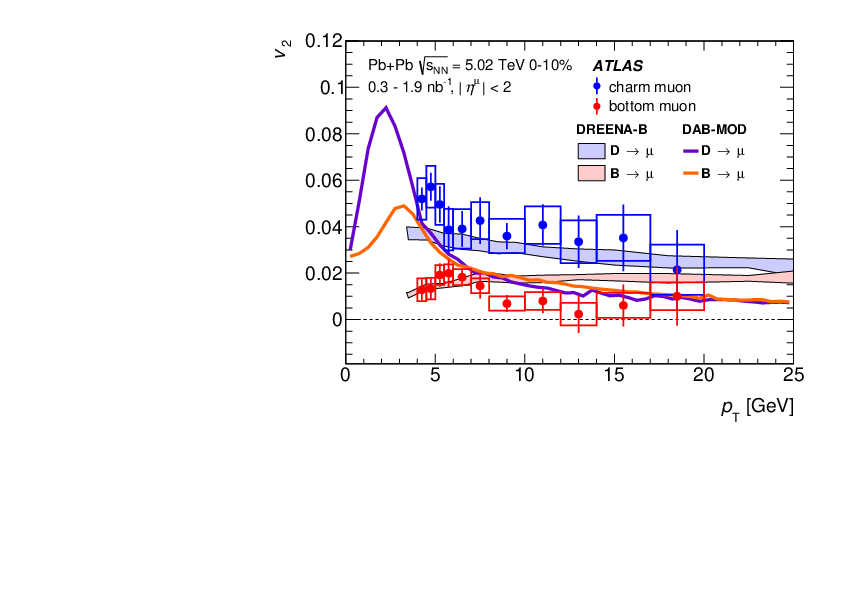
\includegraphics[width=0.485\textwidth]{Figures/Chapter2/ATLASNPMUv2.png}
\caption{The $v_2$ of the electrons from b hadron decays as a function of electron $p_T$ measured by the ALICE experiment (left) and the $v_2$ of the muon from b hadron decays as a function of muon $v_2$ measured by the ATLAS experiment (right) are shown above.}
\label{BeautyEV2}
\end{center}
\end{figure}   


Comparing Figure \ref{BeautyEV2} with Figure \ref{HQV2}, we can see that beauty quarks does not demonstrate as much anisotropy as charm quarks in heavy-ion collision. However, so far, fully reconstructed B-meson $v_2$ has not been measured by any experiment. 




\section{Nuclear Modification Factor}

As mentioned previously, the hadron nuclear modification factor $R_{AA}$ can describe the modification of collisions system compared to the $pp$ collision in the hadron spectra. To study medium modification of heavy quarks, we first would like to investigate the cold nuclear matter effect in $pA$ collisions. Figure \ref{DRPA} and Figure \ref{BRPA} show the prompt D mesons and B mesons nuclear modification factor $R_{pA}$ in pPb collisions measured by the ALICE experiment \ref{ALICEDRPARef} and the CMS experiment \ref{CMSBRPARef} respectfully 



\begin{figure}[hbtp]
\begin{center}
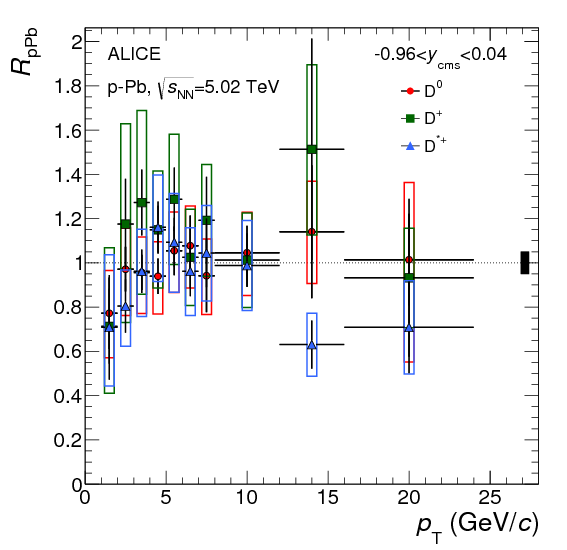
\includegraphics[width=0.60\textwidth]{Figures/Chapter2/ALICEDRpA.png}
\caption{The $R_{pA}$ as a function of $p_T$ of prompt D mesons measured by the ALICE experiment is shown above.}
\label{DRPA}
\end{center}
\end{figure}   

\begin{figure}[hbtp]
\begin{center}
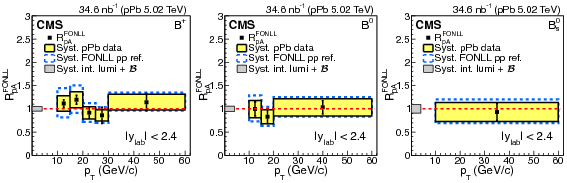
\includegraphics[width=1.10\textwidth]{Figures/Chapter2/CMSDRpA.png}
\caption{The $R_{pA}$ as a function of $p_T$ of $B^+$, $B^0$, and $B^0_s$ mesons measured by the CMS experiment is shown above.}
\label{BRPA}
\end{center}
\end{figure}   

Therefore, we can see that there is no significant modification of the charm quarks in cold nuclear matter since the $R_{pA}$ of $D^0$ is overall unity within experimental uncertainties. Hence, any modification of D-mesons observed in the $AA$ collisions should come from final state QGP effect instead of initial state effect of nPDF of Pb ions. 

Next, we investigate B and D mesons $R_{AA}$ the $AA$ collisions. Figure \ref{HQRAA} $R_{AA}$ heavy flavor hadrons measured with experiments at RHIC and LHC.

\begin{figure}[hbtp]
\begin{center}
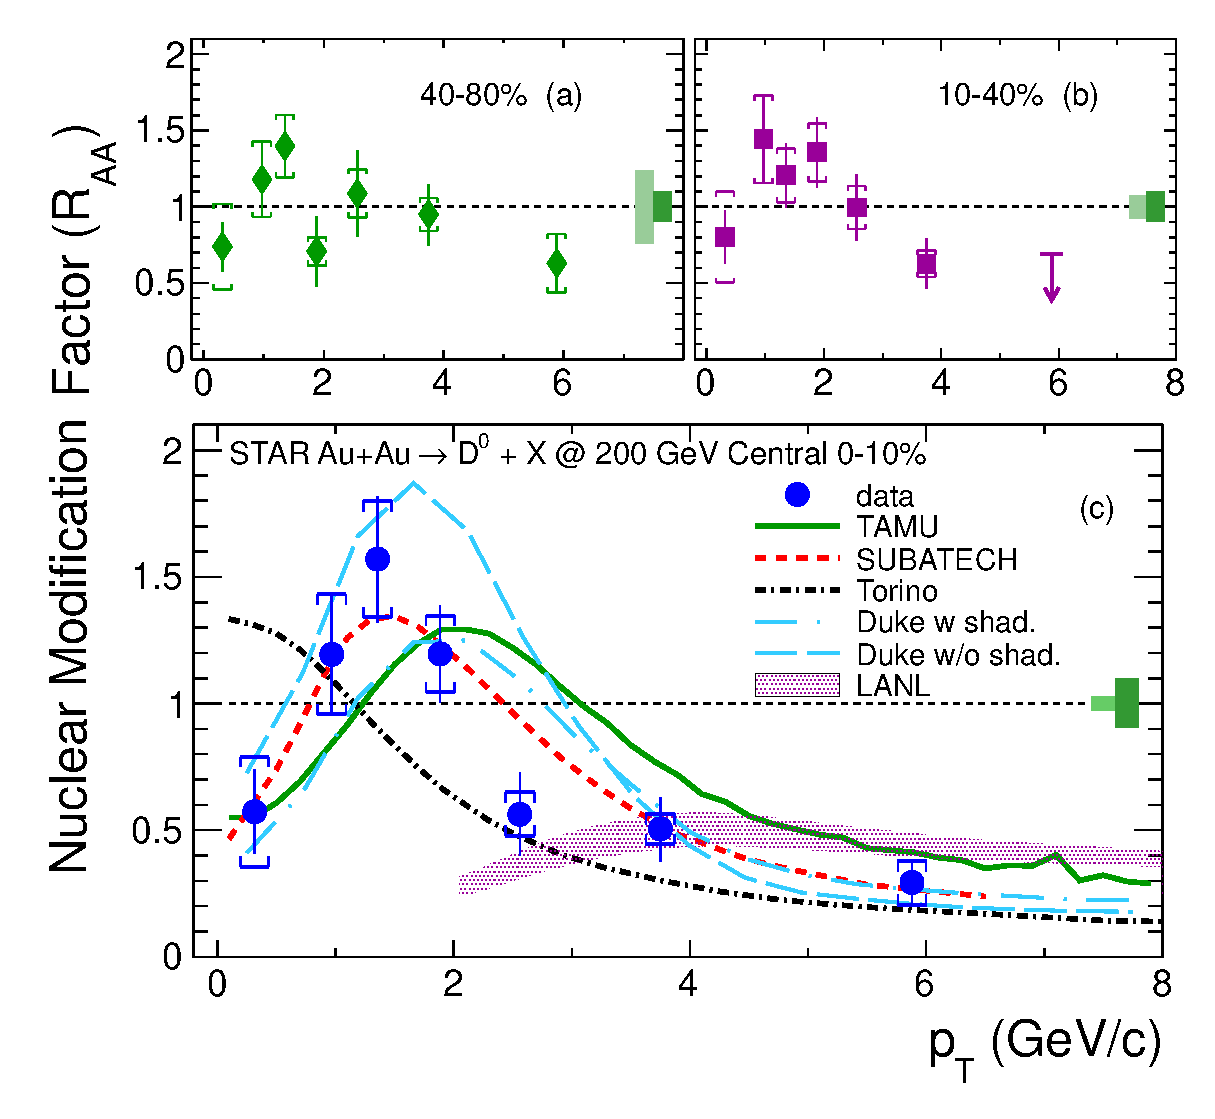
\includegraphics[width=0.47\textwidth]{Figures/Chapter2/STARRAA.eps}
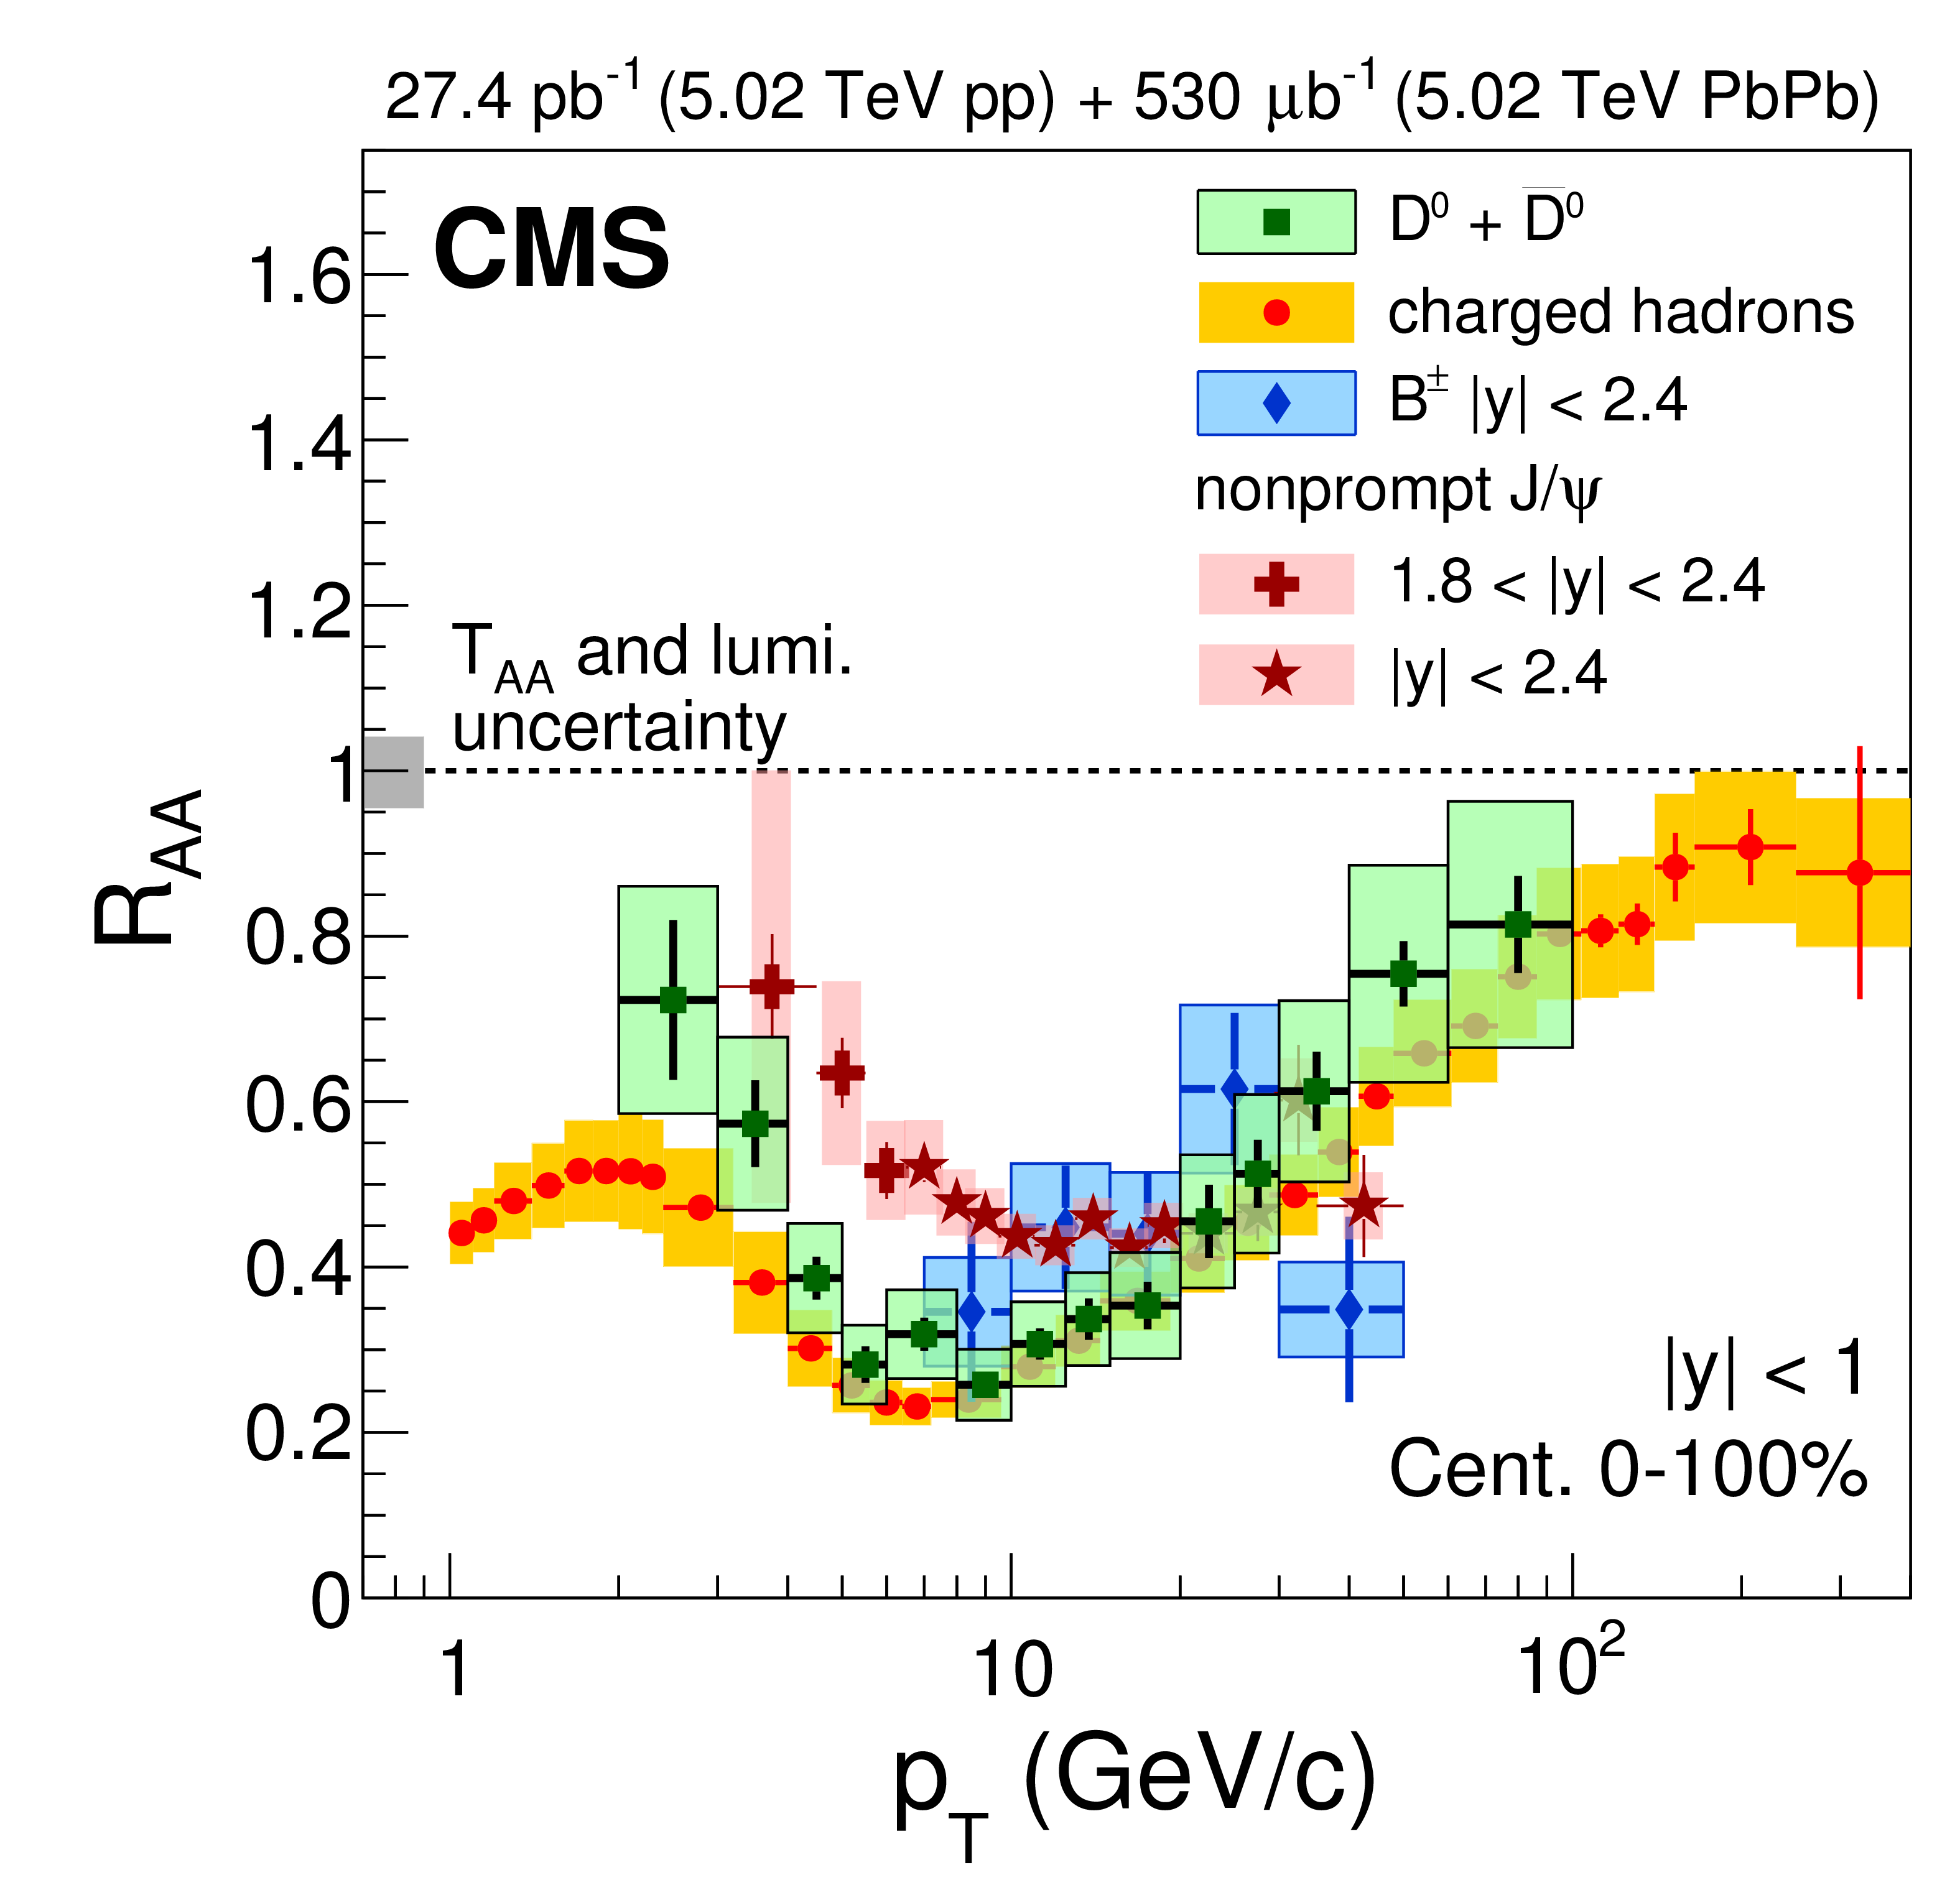
\includegraphics[width=0.47\textwidth]{Figures/Chapter2/CMSRAA.png}
\caption{The $D^0$ $R_{AA}$ vs $p_T$ with the STAR experiment in 0 - 10\%, 10 - 40\%, and 40 - 80\% centrality at RHIC and the $D^0$, $B^+$, non-prompt $J/\psi$ and charged hadrons $R_{AA}$ vs $p_T$ at at 0 - 100\% centrality with the CMS experiment at LHC are shown above.}
\label{HQRAA}
\end{center}
\end{figure}   

We could see that $R_{AA}$ of $D^0$ and $B^+$ are both below 1, which suggest charm and beauty quarks lose a significant fraction of energy to the QGP medium. As $p_T$ increases, the $R_{AA}$ of light and heavy flavor hadrons converge to the same value and approach 1, which Lorentz $\gamma$ factor come into play where the mass of the hadron become irrelevant. In addition, the CMS results above indirectly agree with the expectation of the flavor dependence of energy loss: $R_{AA}^{h} < R_{AA}^{D} < R_{AA}^{B} < 1$. The $R_{AA}$ results are in reasonable agreement with most theoretical model calculations. 

To better constrain theoretical model calculations and understand the interaction mechanism of heavy quarks with the QGP medium, we need to perform more precise measurements of B and D mesons $R_{AA}$ and $v_2$ down to lower $p_T$ where the mass heavy quarks become important and theory diverge. The ALICE experiment has performed measurement of prompt and non-prompt D mesons $R_{AA}$ down to very low $p_T$ shown in Figure \ref{ALICEDRAALow} below


\begin{figure}[hbtp]
\begin{center}
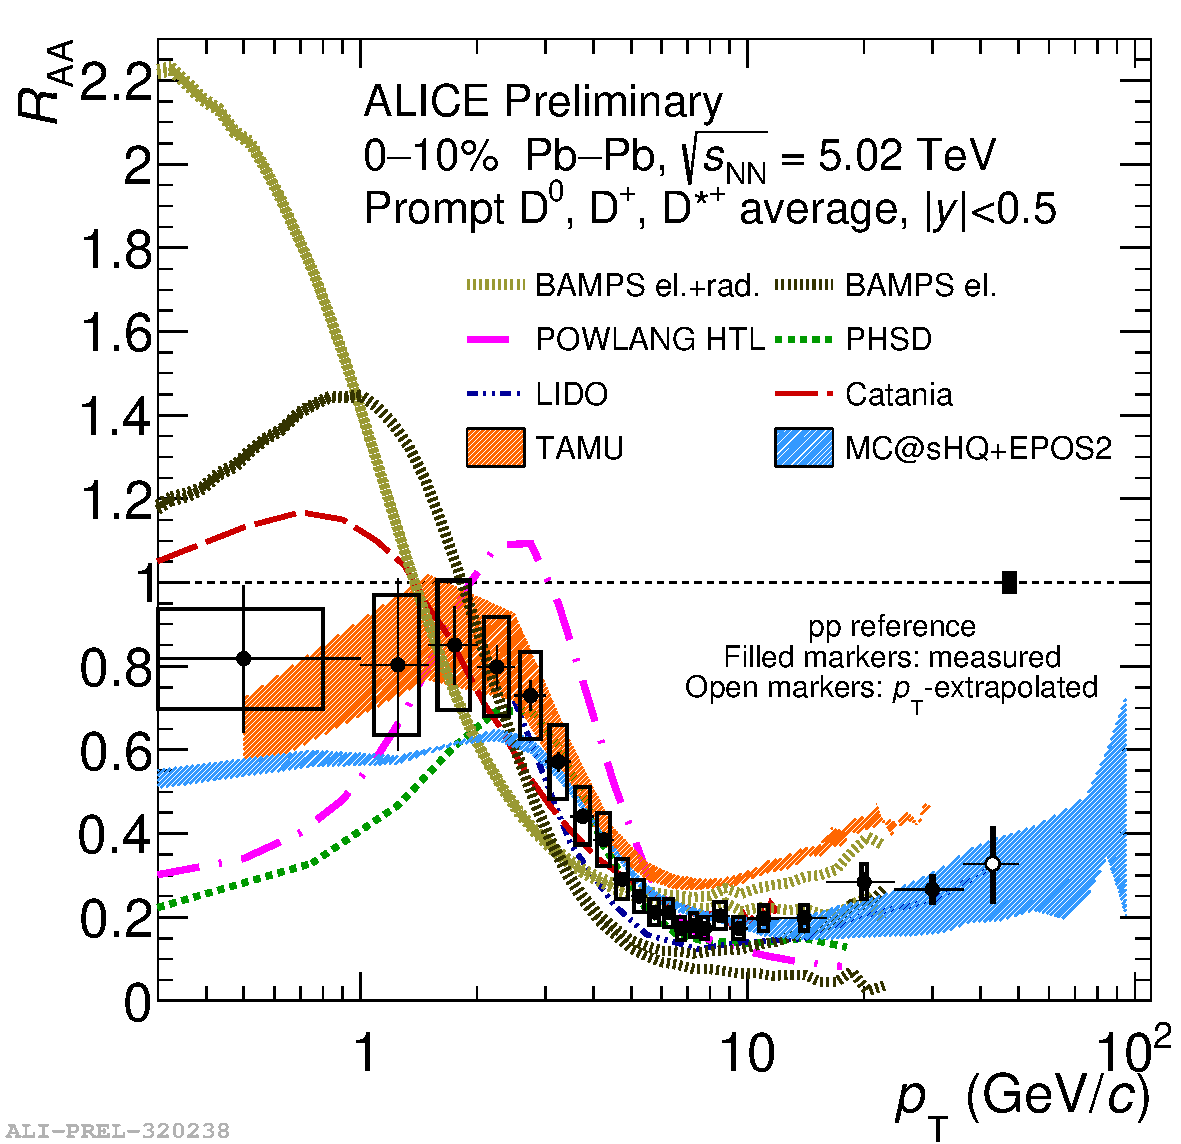
\includegraphics[width=0.48\textwidth]{Figures/Chapter2/ALICEDRAALow.pdf}
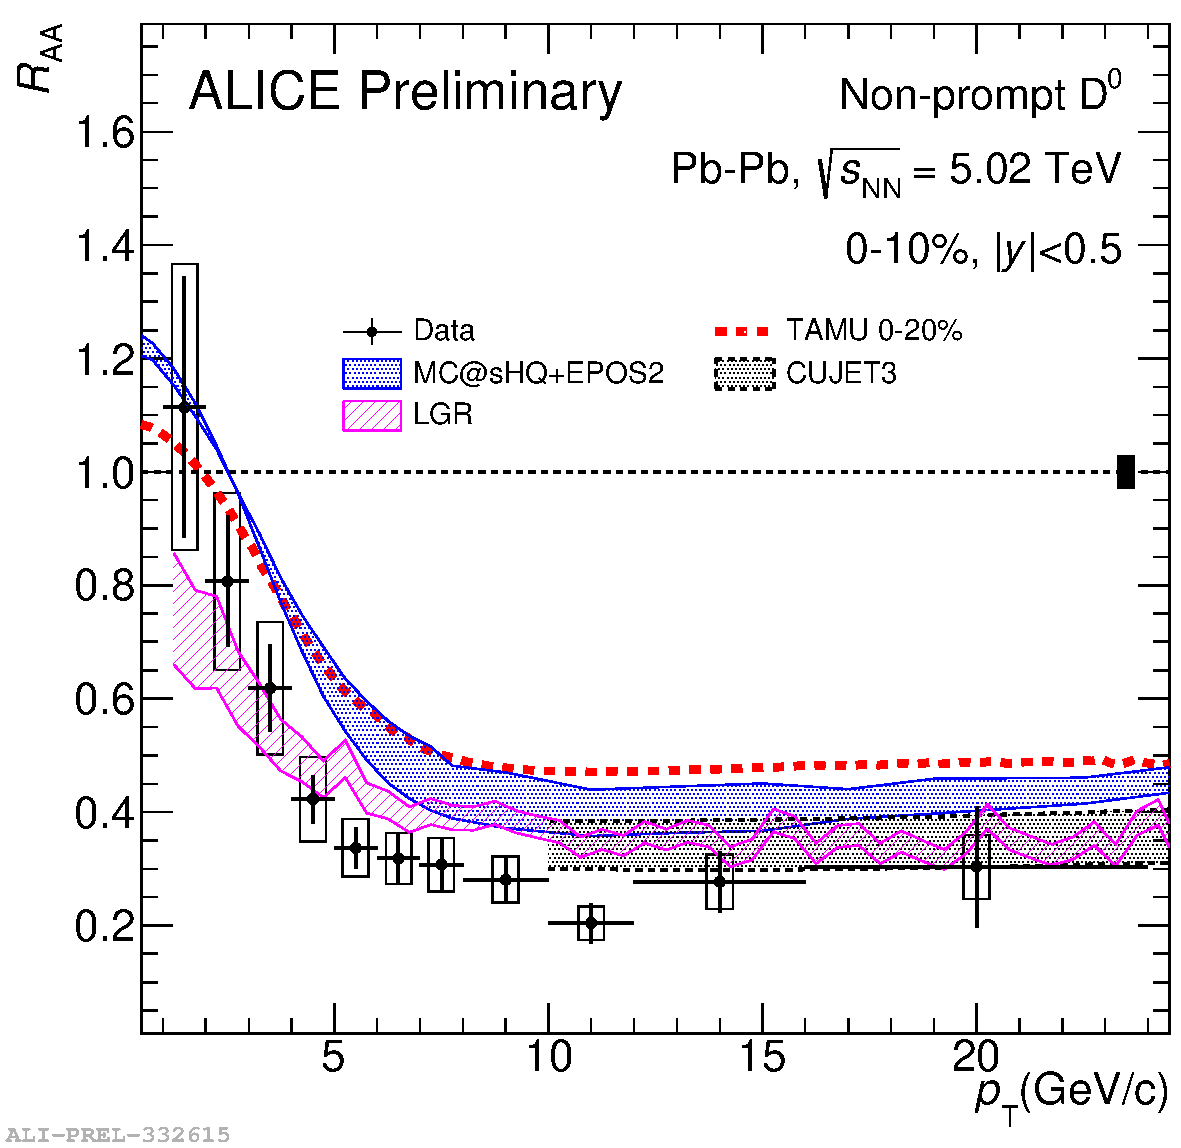
\includegraphics[width=0.48\textwidth]{Figures/Chapter2/ALICENPDRAALow.pdf}
\caption{The prompt D mesons $R_{AA}$ vs $p_T$ down to $p_T = 0$ (left) and non-prompt D mesons down to $p_T = 1$ GeV/c (right) are shown above.}
\label{ALICEDRAALow}
\end{center}
\end{figure}   

From the ALICE measurement of prompt and non-prompt D mesons $R_{AA}$ down to very low $p_T$, we could see that very few model can simultaneously describe $D^0$ $R_{AA}$ at both low and high $p_T$. Nonetheless, the fully reconstructed B meson $R_{AA}$ from exclusive b decay down to very low $p_T$ is still missing. We should try to perform B meson $R_{AA}$ measurement down to low $p_T$ to provide a complete picture to help understand and probe the QGP at longer wavelengths. Also, good to measure inclusive beauty production cross section in pp collisions to test pQCD calculations.  



\section{Production Yield Ratio}

According to the theoretical reviews of heavy quarks hadrochemistry in heavy-ion collisions \cite{StrangetoLight,BaryontoMeson}, the strange-to-non-strange meson ($H_s/H^0$) and baryon-to-meson ($\Lambda_{Q}/H^{0}$) ratios are excellent observables to test hadronization models. Both RHIC and LHC have carried out extensive measurements fully reconstructed charm hadron yield ratios. Figure \ref{HadroPlotCharm} shows the fully reconstructed prompt $D^+_s/D^0$ ratio measured by the STAR \cite{} and ALICE \cite{} experiments


\begin{figure}[hbtp]
\begin{center}
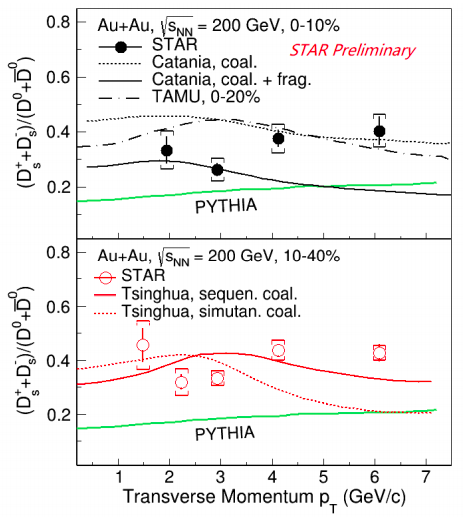
\includegraphics[width=0.30\textwidth]{Figures/Chapter2/STARDsD0.png}
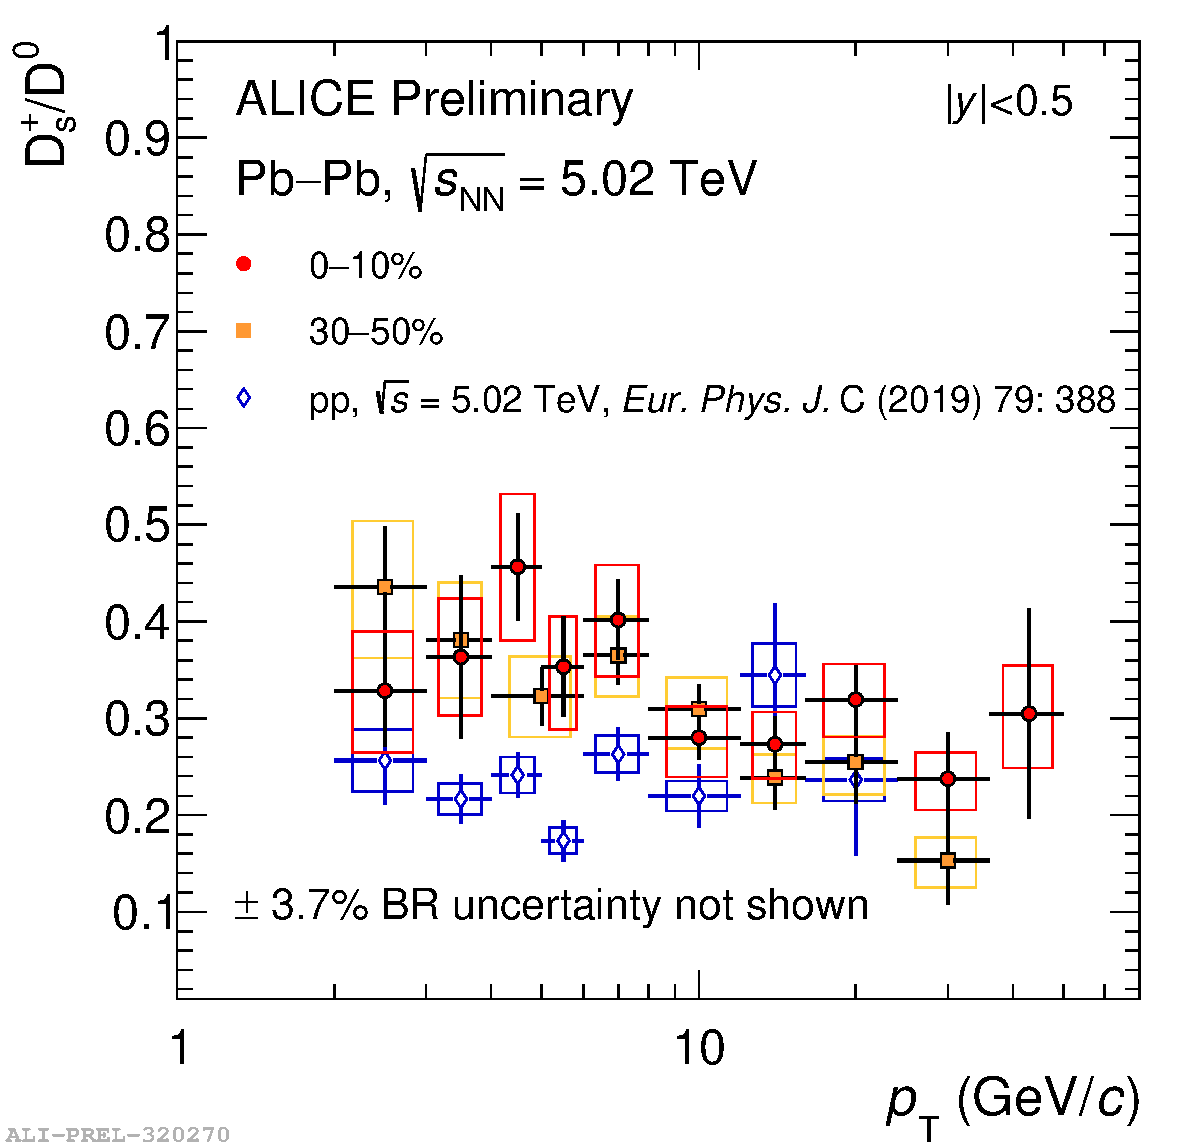
\includegraphics[width=0.41\textwidth]{Figures/Chapter2/ALICEDsD0.pdf}
\caption{The fully reconstructed $D_s^+/D^0$ ratio in Au + Au measured by the STAR experiment at RHIC (left) and in PbPb the ALICE experiment at LHC (right) as functions of $p_T$ are shown above.}
\label{HadroPlotCharm}
\end{center}
\end{figure}   



Figure \ref{HadroPlotCharm} shows the fully reconstructed $\Lambda_C^+/D^0$ ratio measured by the STAR and ALICE experiments



\begin{figure}[hbtp]
\begin{center}
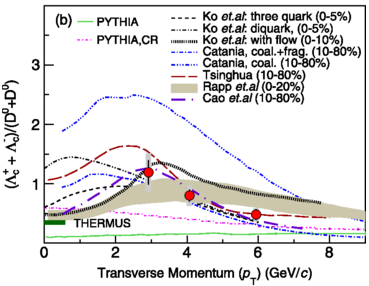
\includegraphics[width=0.48\textwidth]{Figures/Chapter2/STARLambdaCD0.png}
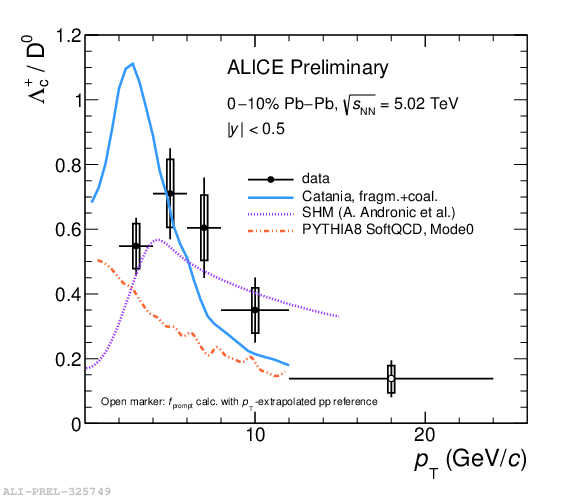
\includegraphics[width=0.48\textwidth]{Figures/Chapter2/ALICELambdaCD0}
\caption{The fully reconstructed $\Lambda_C^+/D^0$ ratio in pp and heavy-ion collisions measured by the STAR experiment at RHIC (left) and the CMS experiment at LHC (right) are shown above.}
\label{HadroPlotCharm}
\end{center}
\end{figure}   

\clearpage


The ALICE experiment also performs a comprehensive study on charm quark hadronization in pp, pPb, and PbPb. Figure \ref{ALICEMulti} shows the $D^+_s/D^0$ and $\Lambda_c/D^0$  ratios as functions of event multiplicity from small to large collision systems. 

\begin{figure}[hbtp]
\begin{center}
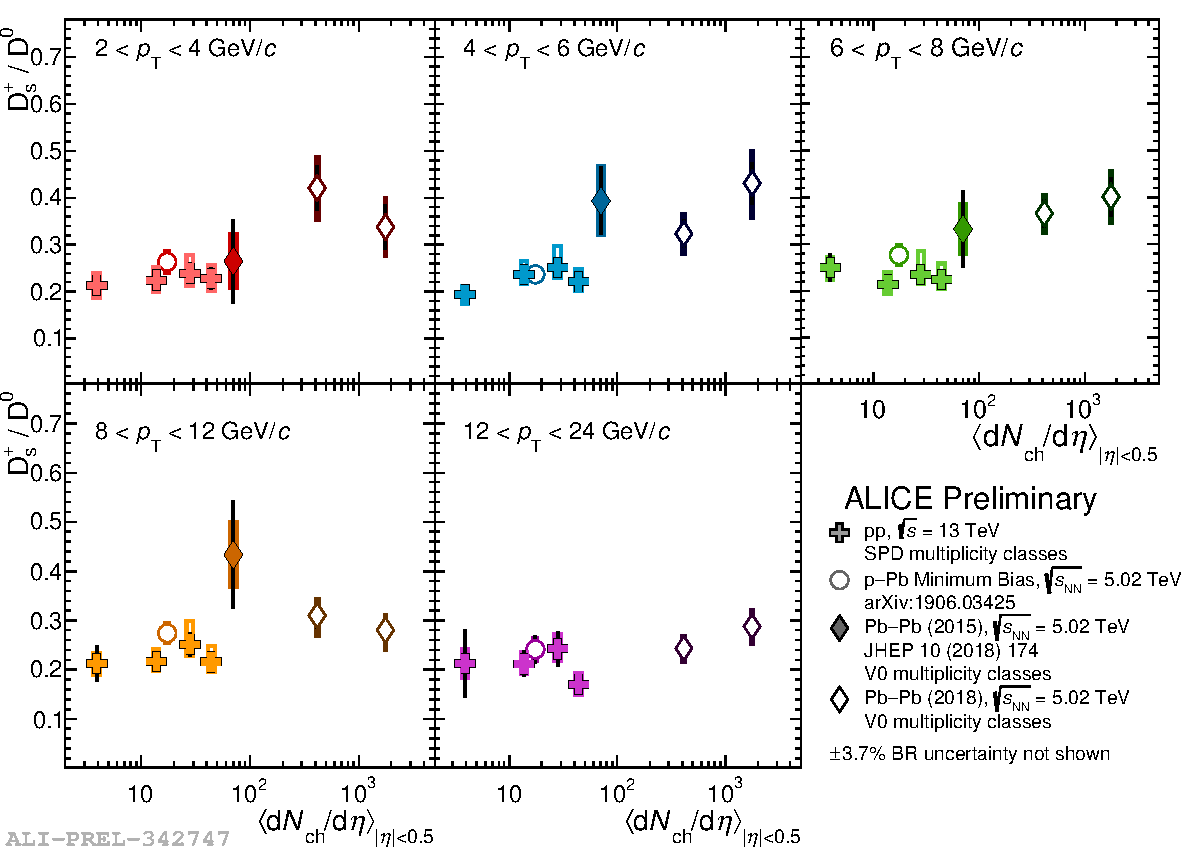
\includegraphics[width=0.80\textwidth]{Figures/Chapter2/ALICEDsD0Multi.pdf}
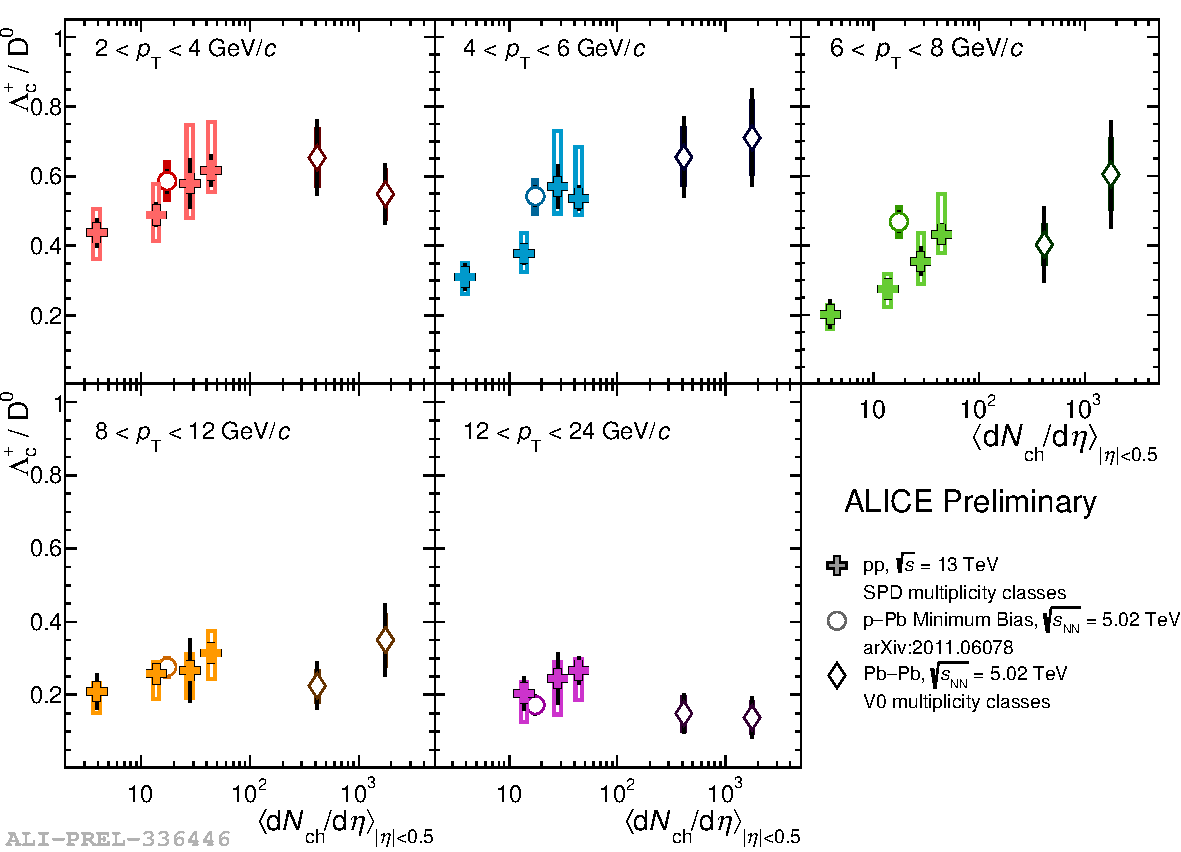
\includegraphics[width=0.80\textwidth]{Figures/Chapter2/ALICELambdaD0Multi.pdf}
\caption{The fully reconstructed $D^+_s/D^0$ (top) and $\Lambda_C^+/D^0$ ratio (botton) as a function of event multiplicity $\langle dN_{ch}/d\eta \rangle$ within $|\eta| < 0.5$ in $p_T$ from 2 - 4, 4 - 6, 6 - 8, 8 - 12, and 12 - 24 GeV/c in pp, pPb, and PbPb collisions measured by the ALICE experiment are shown above.}
\label{ALICEMulti}
\end{center}
\end{figure}   





We can see that in general, $D_s^+/D^0$ while $\Lambda_C^+/D^0$ ratio in heavy-ion collisions lies above its ratio in $pp$ collisions. From the multiplicity studies, we see an increasing trend of both $D^0_s/D^0$ and $\Lambda_C^+/D^0$ ratios. Many different theoretical predictions agree reasonably well with the experiments due to their large uncertainties. However, such large discrepancies among hadronization models significantly limit our ability to interpret heavy flavor experimental data. Moreover, this is only in the charm sector, such fully reconstructed b-hadron measurements to study beauty hadrochemistry are still missing. 


%Bs/B+



Therefore, it is crucial to have more precise measurement over a wide range of $p_T$ and multiplicity in both beauty and charm sectors to constrain theoretical models. Currently, the only published fully reconstructed b-hadron measurement in heavy-ion collision is the $B^0_s/B^+$ based on CMS 2015 PbPb data set \ref{CMSBsBP2015}. Figure \ref{BsBP2015} shows the $B^0_s/B^+$ $R_{AA}$ ratio in pp and PbPb collisions

\begin{figure}[hbtp]
\begin{center}
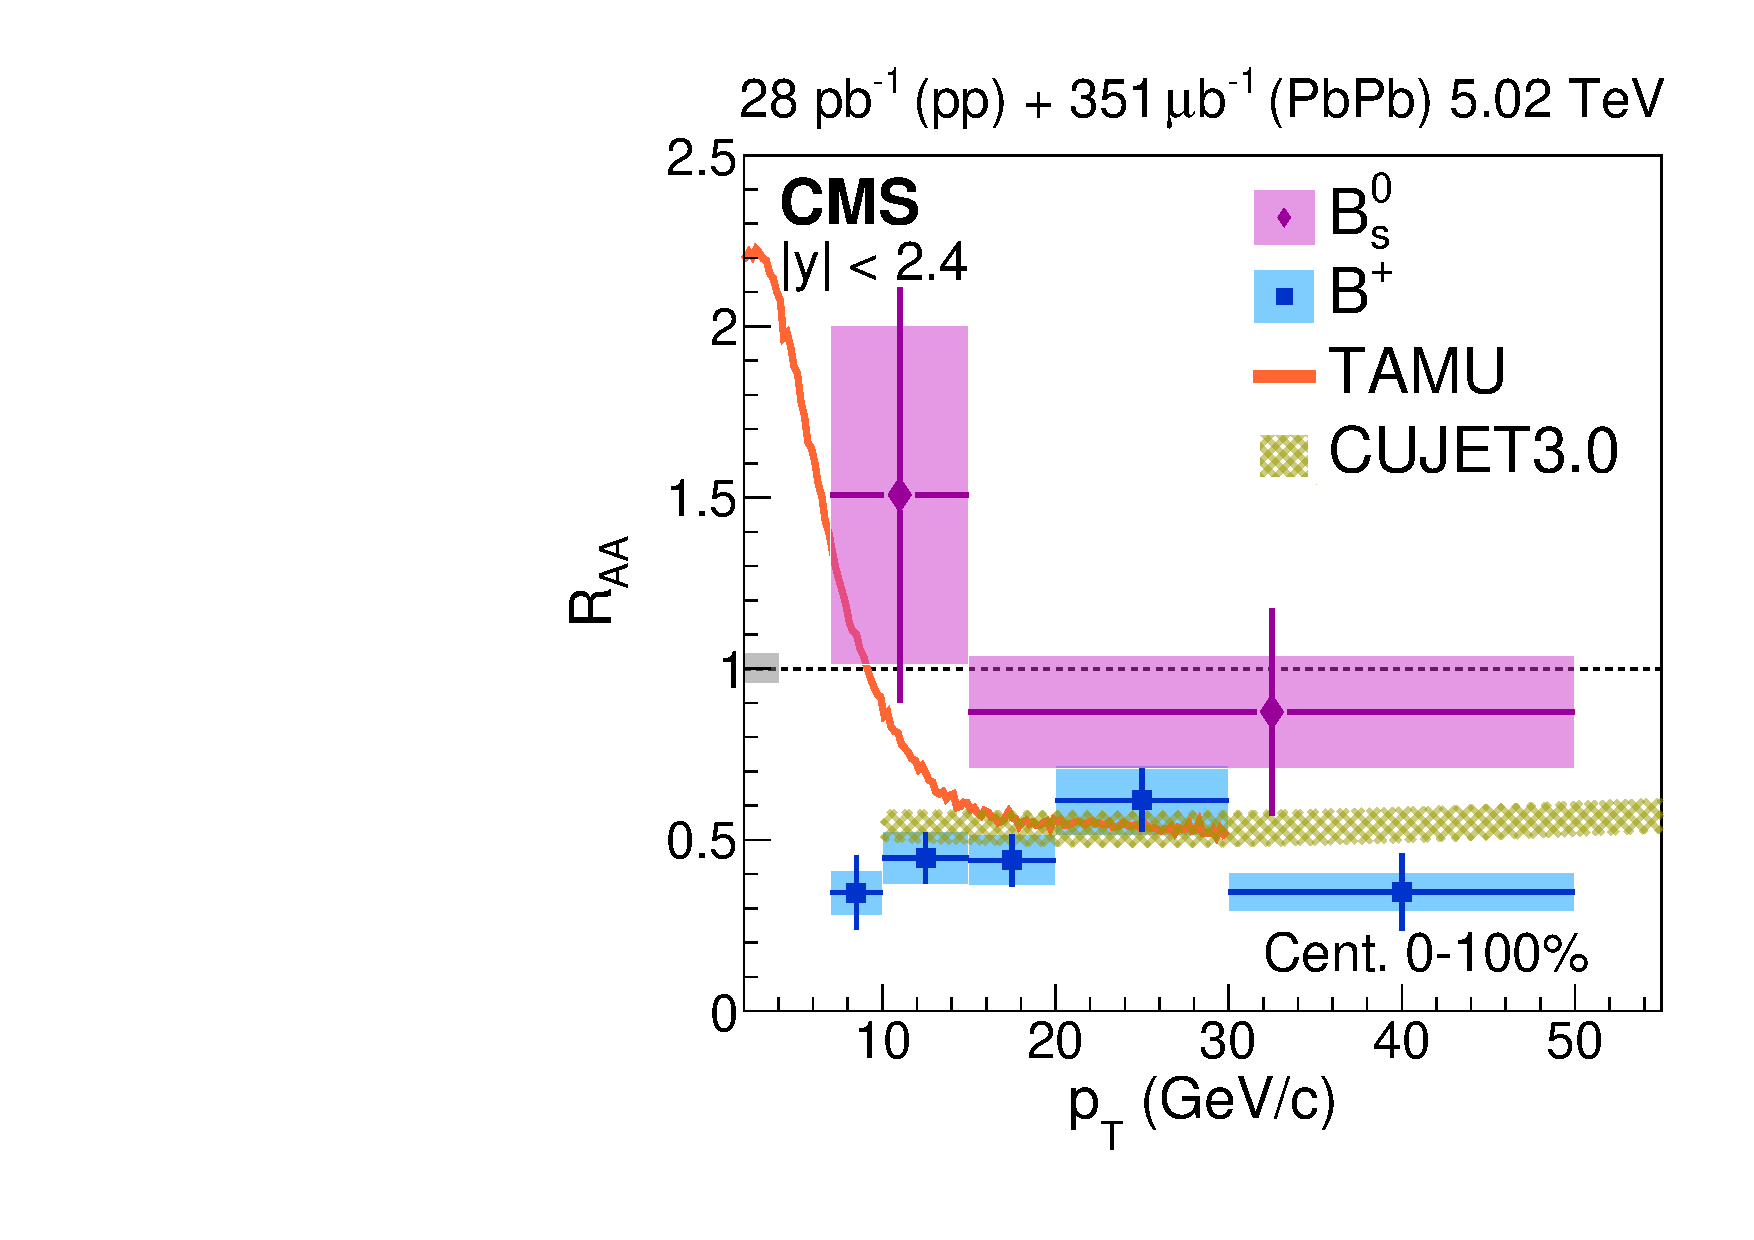
\includegraphics[width=0.48\textwidth]{Figures/Chapter2/CMSBsBPRAA2015.pdf}
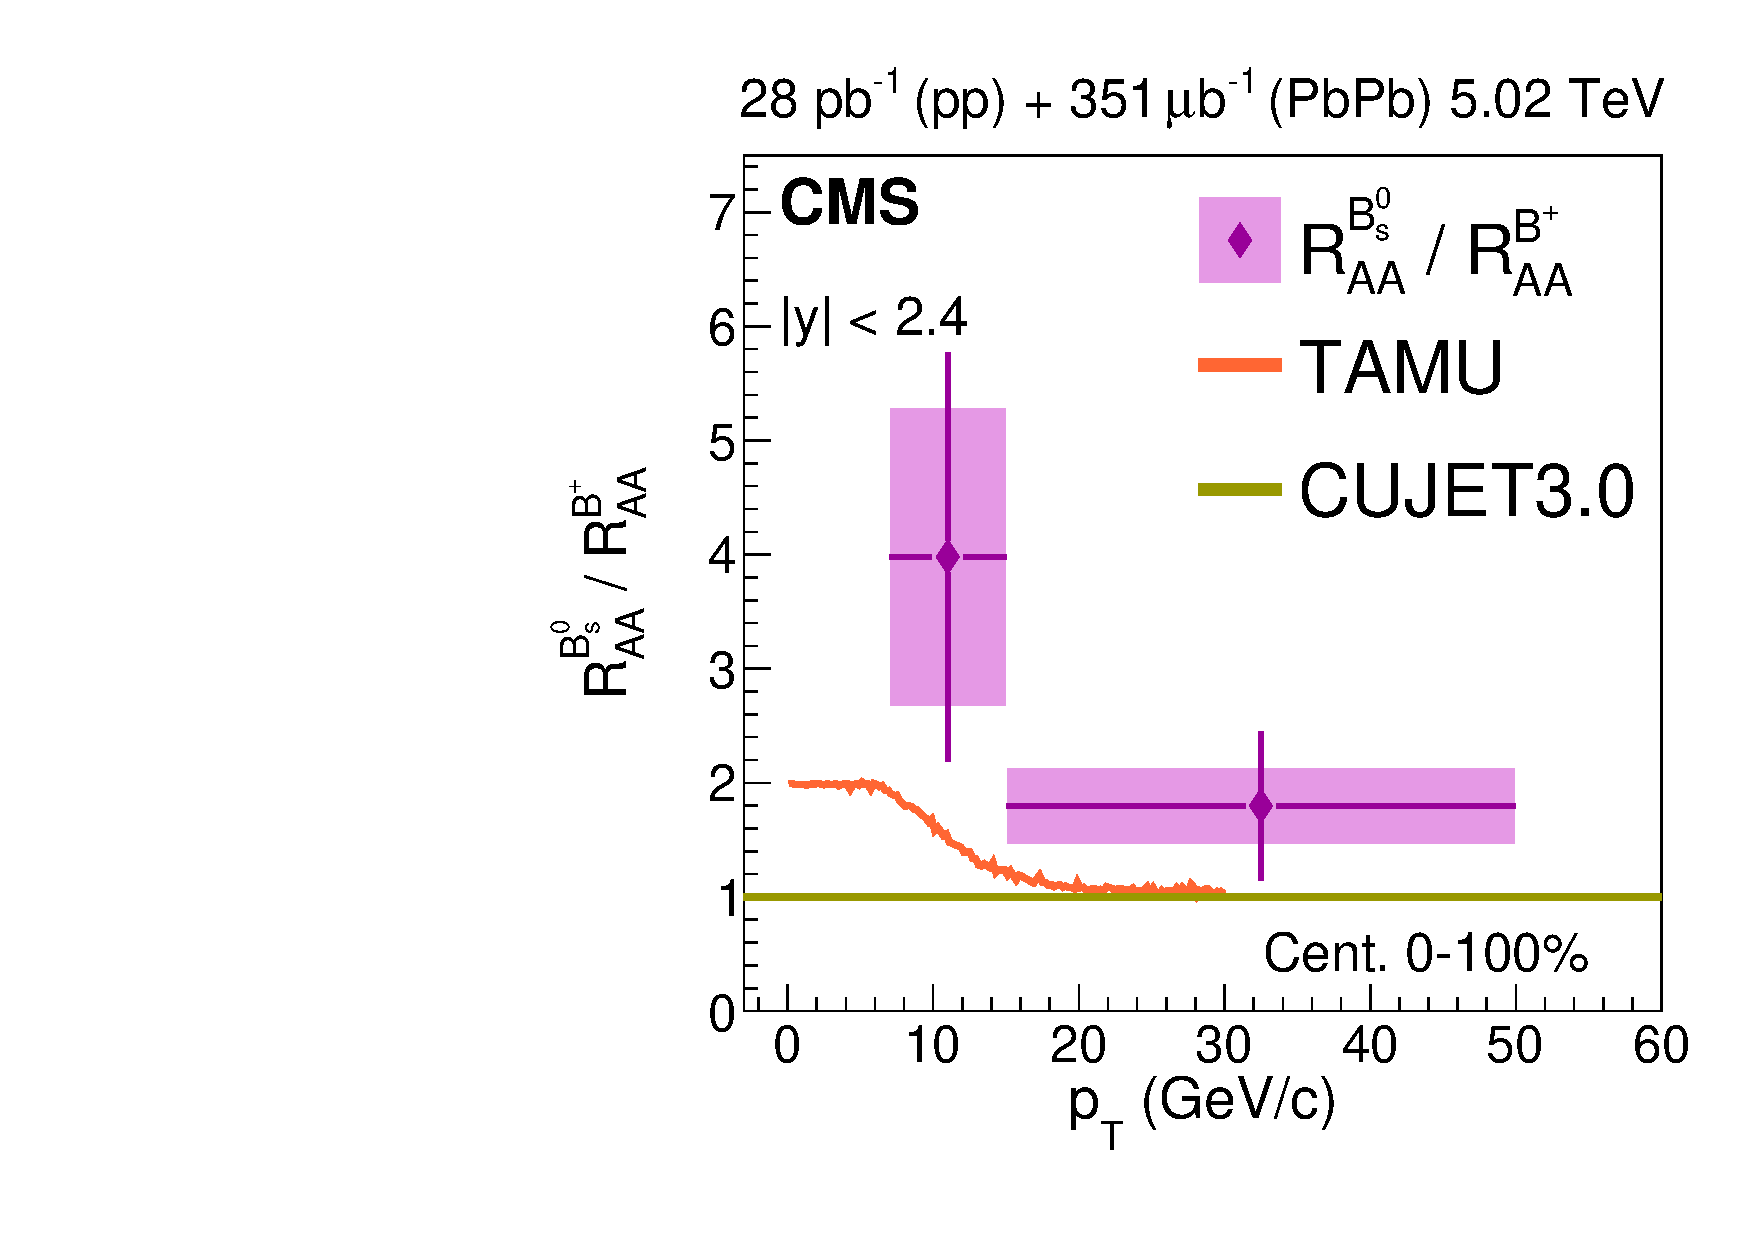
\includegraphics[width=0.48\textwidth]{Figures/Chapter2/CMSBsBP2015.pdf}
\caption{The fully reconstructed $B^0_s$ and $B^+$ $R_{AA}$ (left) and $B^0_s/B^+$ $R_{AA}$ ratio (right) as a function of $p_T$ using the 2015 CMS pp and PbPb datasets are shown above.}
\label{BsBP2015}
\end{center}
\end{figure}   

This first fully reconstructed B-meson measurement in heavy-ion collision is good. Nevertheless, the measure has relatively large uncertainties. The $B^0_s$ significance is still below 5 $\sigma$. In order to better constrain model calculations and better, we should perform more differentiated measurement with improved precision. 

In the baryon-to-meson ratio studies, LHCb has conducted fully reconstructed $\Lambda_b/B^+$ ratio in pp and pPb collision \cite{LHCbLambdaB} shown below in Figure \ref{LHCbLambda}


\begin{figure}[hbtp]
\begin{center}
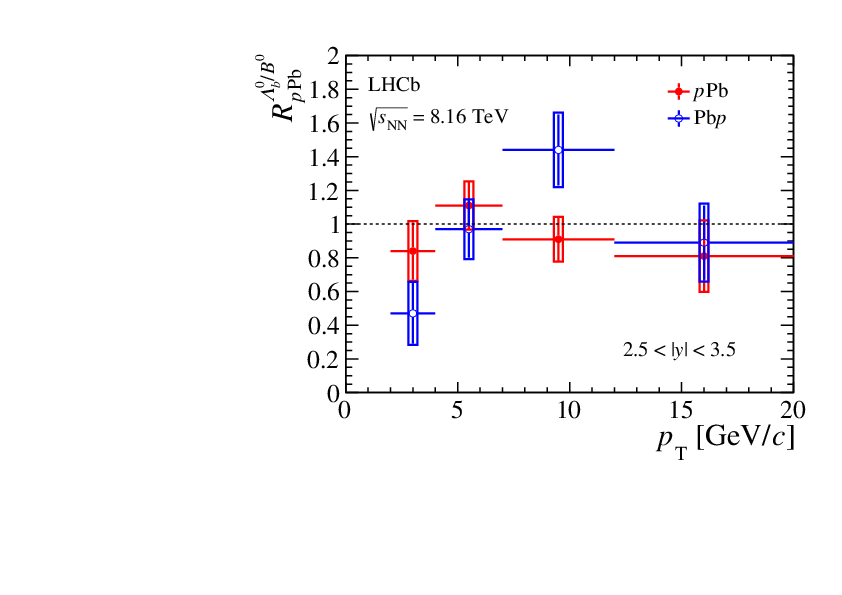
\includegraphics[width=0.60\textwidth]{Figures/Chapter2/LHCbRpPb.png}
\caption{The fully reconstructed $\Lambda_b/B^+$ $R_{pA}$ ratio as a function $p_T$ and $y$ in pp, pPb, and Pbp collisions measured by the LHCb experiment are shown above.}
\label{LHCbLambda}
\end{center}
\end{figure}   


We can see a  $\Lambda_b$ in the forward region from LHCb measurement. It would be interesting to conduct similar measurement in the mid-rapidity region in pp and pPb collision. However, so far no fully reconstructed $\Lambda_b$ measurement have been carried out in heavy-ion collisions due to the limited statistics and large combinatorial background of $\Lambda_b$. 

\section{Heavy Flavor Hadron-Jet Angular Correlations}

Aside traditional heavy flavor observables: $R_{AA}$, $v_{2}$, and cross section ratio, modern observables, such as heavy flavor hadron-hadron and heavy flavor hadron-jet angular correlations, have higher differentiation to provide more insight to understand the dynamics and interaction mechanism of heavy quarks in the QGP medium. The measurements of angular correlations between heavy flavor hadrons and jets can be used to constrain parton energy loss mechanisms and to better understand the heavy-quark diffusion inside the medium. From the D-jet angular correlation, we can quantify the medium modification to the radial profile of charm quarks and shed light on the interaction mechanism of charm quark with the medium. Figure \ref{DJETCorr} shows the measurement of D-jet angular correlation in PbPb and pp collisions with the CMS experiment \cite{CMSDJet}

\begin{figure}[hbtp]
\begin{center}
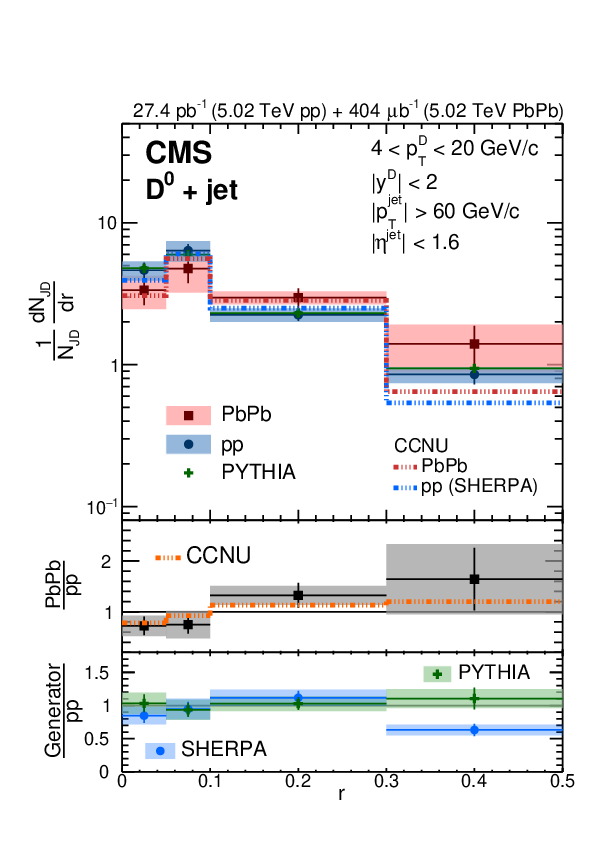
\includegraphics[width=0.48\textwidth]{Figures/Chapter2/CMSDJetLow.png}
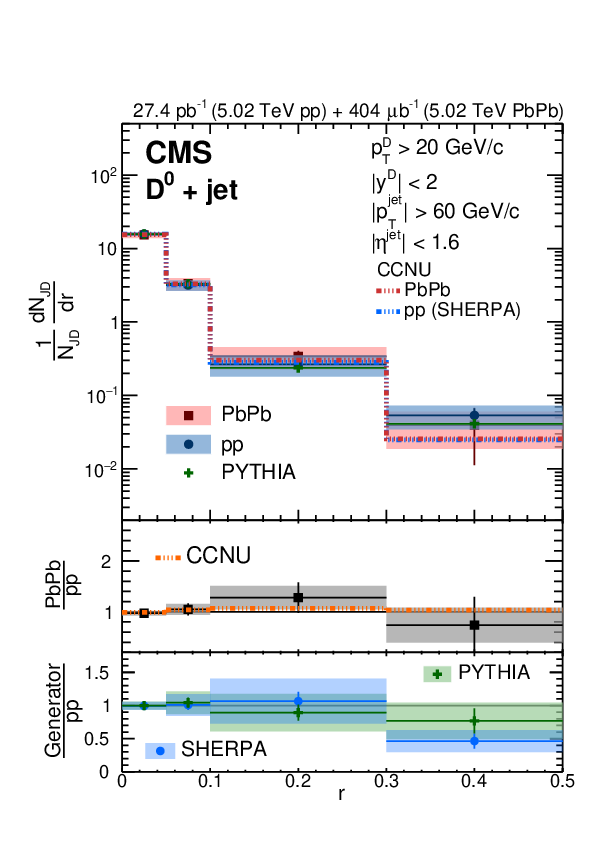
\includegraphics[width=0.48\textwidth]{Figures/Chapter2/CMSDJetHigh.png}
\caption{Distributions of fully reconstructed $D^0$ mesons in jets, as a function of the distance from the jet axis ($r$) for jets of $p_T^{jet} >$ 60 GeV=c and $|\eta^{jet}| <$ 1.6
measured in pp and Pb-Pb collisions at $\sqrt{s_{NN}} = $ 5.02 TeV, for $4 < p_T^D < 20$ GeV/c and $p_T^D > 20$ GeV/c are shown above. The jet radius is defined as $r = \sqrt{(\Delta \phi_{jD})^2 +  (\Delta \eta_{jD})^2 }$ where $\phi_{jD}$ and $\eta_{jD}$ are the $\eta$ and $\phi$ of the $D^0$ meson with respect to the jet axis.}
\label{DJETCorr}
\end{center}
\end{figure}   

We can see that the $D^0$ meson production is pushed radially outward in PbPb collisions compared to pp, which shows effects of charm quark diffusion with the present of the QGP medium. While the CCNU model is in reasonably good agreement with the PbPb/pp ratio, its prediction is lower when compare to measurement of $\frac{1}{N_{jD}}\frac{dN_{jD}}{dr}$ pp and PbPb collisions.

\section{Heavy Flavor Hadron-Hadron Correlations}

Another observable is heavy flavor hadron-hadron correlation, which is even better to tag the heavy quark $Q\bar Q$ pair the produced back to back in the early stage of hard scattering processes and understand the modification effect as they propagate thorough vacuum and medium. Experimentally, the observable is a fully reconstructed open heavy flavor hadron correlate with associated hadrons produced within the same event and subtract the background in mixed events. In the analysis, $\Delta \eta and \Delta \phi$ distributions of the heavy flavor hadron from associated hadron are used to quantify the correlation. Figure \ref{ALICEDHadron} shows the D meson-hadron angular correlation measured with the ALICE experiment \cite{DHadronRef}


\begin{figure}[hbtp]
\begin{center}
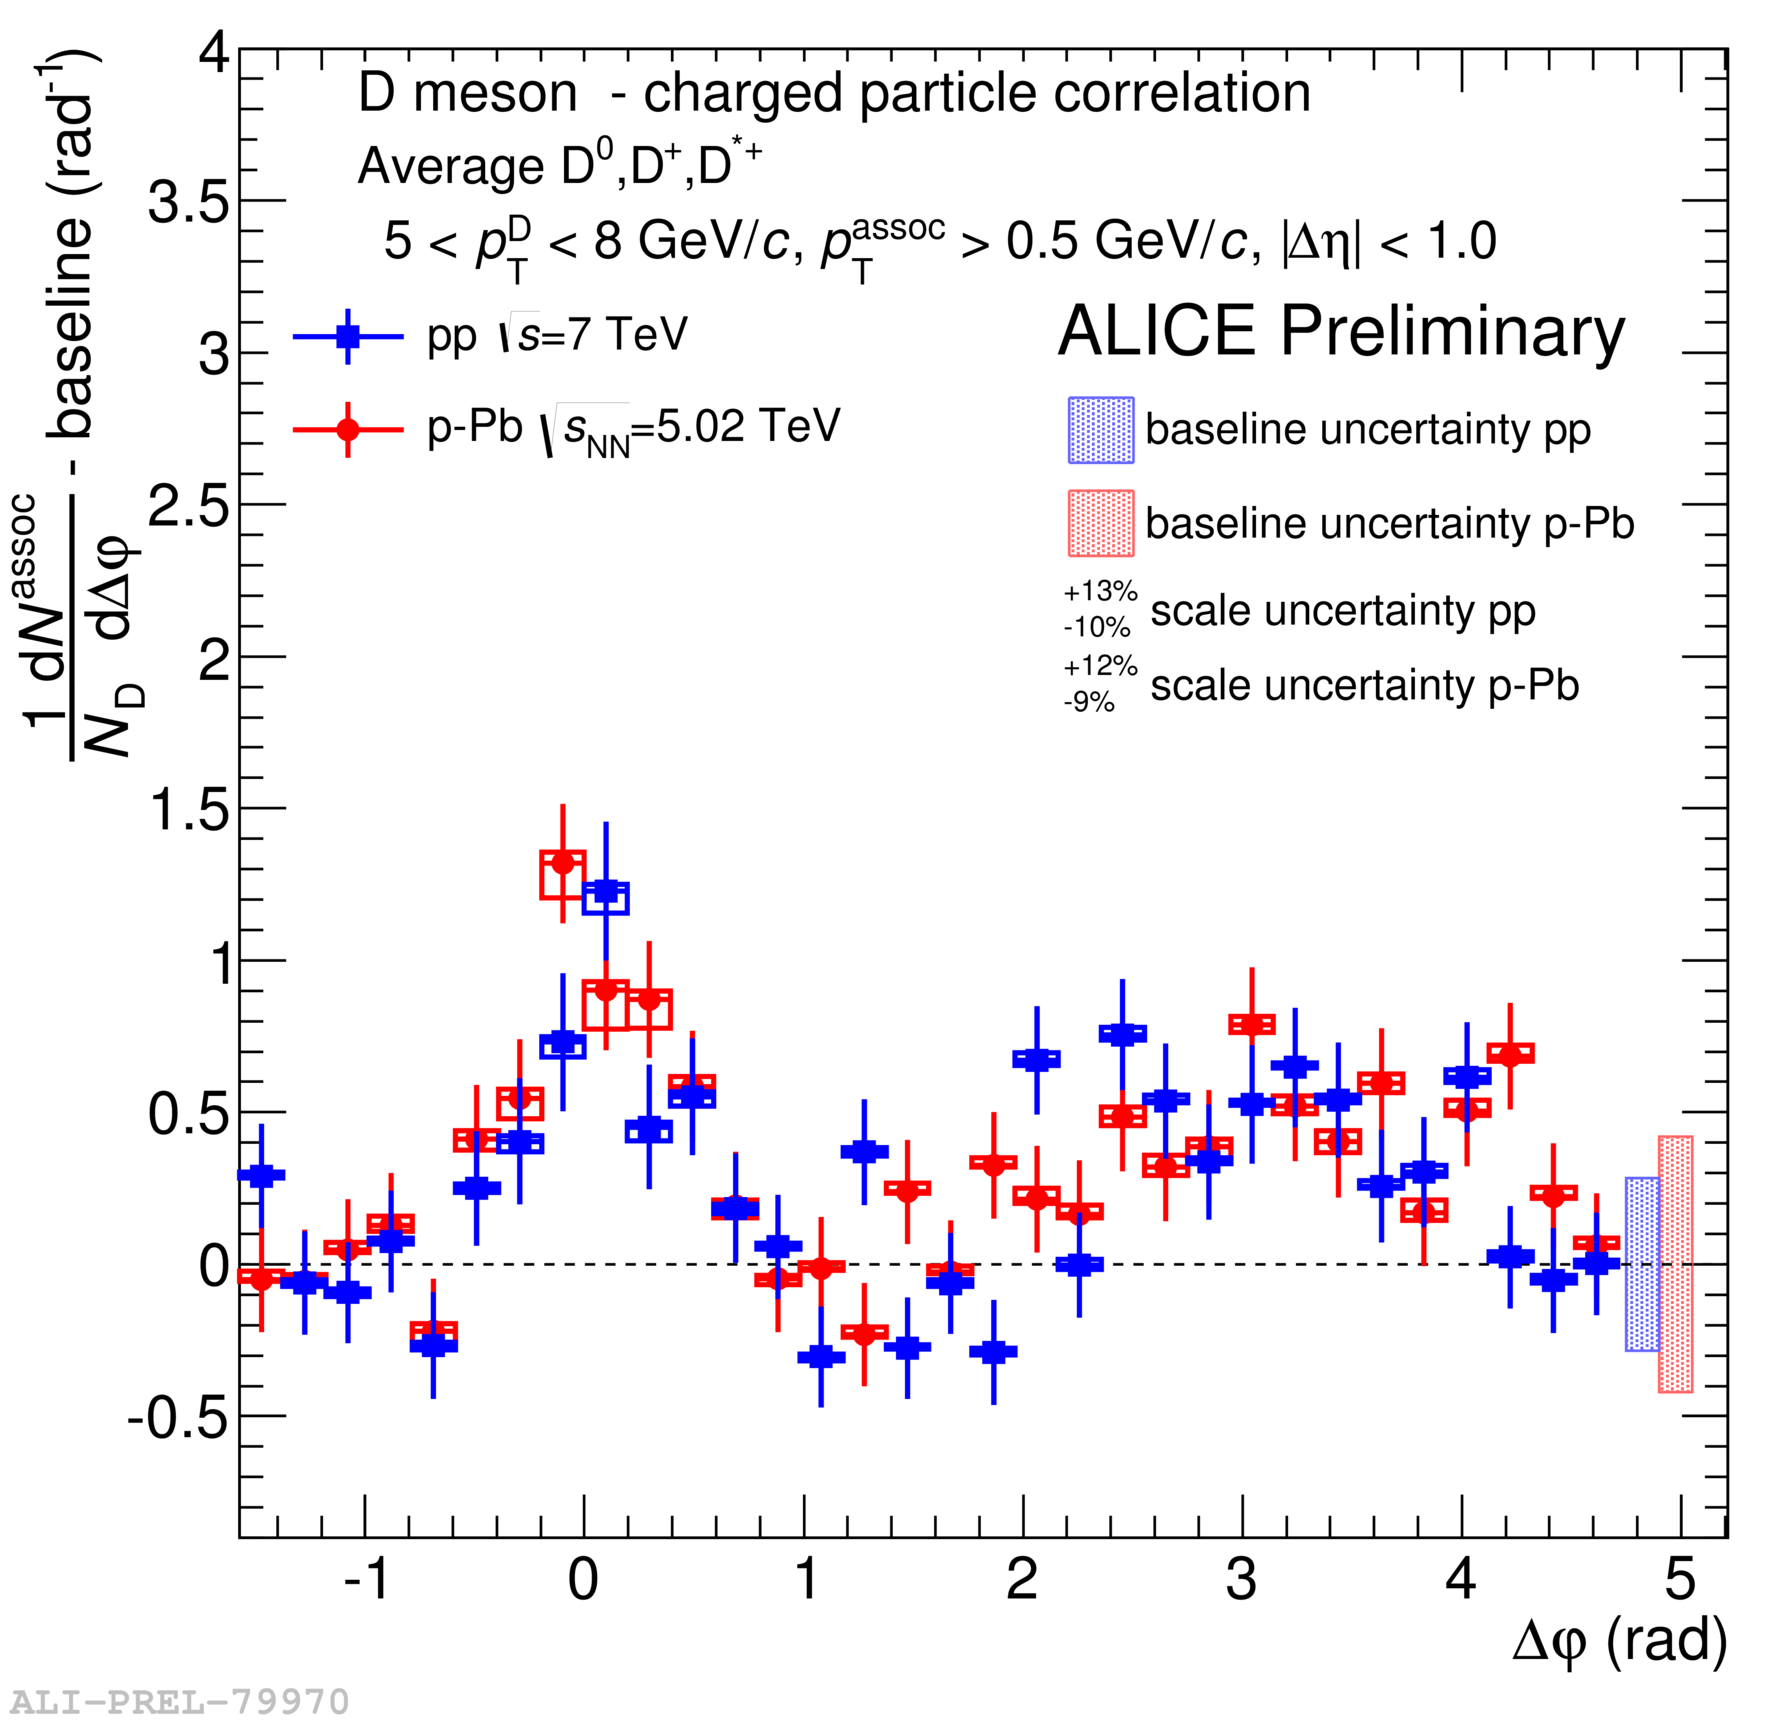
\includegraphics[width=0.48\textwidth]{Figures/Chapter2/ALICEDHadron.png}
\includegraphics[width=0.48\textwidth]{Figures/Chapter2/ALICEDHadronPP.png}
\caption{The ALICE D-hadron angular correlated in both pp (blue) and pPb (red) collision (left) and the comparison of pp data with PYTHIA calculations (right) are shown above.}
\label{ALICEDHadron}
\end{center}
\end{figure}   

In the D-hadron correlation, there are two peaks at $\Delta \phi =$ 0 and $\pi$. At $\Delta \phi = $0, hadron are produced along with the charm quark via fragmentation mechanism. At $\Delta \phi = \pi$, the hadron are produce from back-to-back jets the to maintain momentum conservation. The pp measurements are overall consistent to PYTHIA calculations. From the comparison of the results in the pp and pPb, the D-hadron angular correlation distribution are compatible with each other with uncertainties. Consequently, no evident effects on the
charm fragmentation and hadronization due to cold nuclear matter can be claimed. 

STAR has perform the 2D $\Delta \eta \time \Delta \phi$ measurement of fully reconstructed $D^0$-hadron correlation in Au + Au collision shown in Figure \ref{STARDHadron}

\begin{figure}[hbtp]
\begin{center}
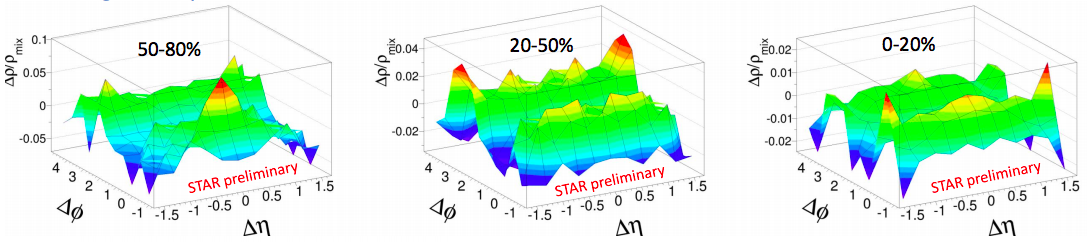
\includegraphics[width=0.80\textwidth]{Figures/Chapter2/STARDHadron.png}
\caption{The 2D $\Delta \eta \time \Delta \phi$ distributions of $D^0$ meson and associated hadrons in Au + Au collision centrality 0 - 20\%, 20 - 50\%, and 50 - 80\% at $\sqrt{s_{NN}} = $ 200 GeV measured by STAR experiment are shown above.}
\label{ALICEDHadron}
\end{center}
\end{figure} 

As expected, the $D^0$-hadron angular correlation get broaden and the peak near $\pi$ disappear in more central Au + Au collisions because QGP are more likely to create and redistribute the energy among particles. In the beauty sector, so far there is no such measurement carried out in heavy-ion collision. The B-hadron correlation measurement, along with the D-hadron correlation measurement, will be crucial to provide deeper insights on heavy quark diffusion and energy loss in the QGP medium. 


\section{Open Question in Heavy Flavor Physics}

As seen in section 2.3, extensive studies on fully reconstructed charm hadrons have been carried out at RHIC and the LHC. In addition, many measurements of fully reconstructed b-hadrons produced in pp and pPb collisions have been carried out by LHCb experiment. In heavy-ion collision, only one measurement of fully reconstructed b-hadron has also been published. Hence, to have a more comprehensive understanding of heavy flavor physics, we should perform more precise and differential measurement on fully reconstructed b-hadrons. 

%The ALICE experiment also performs a comprehensive study on charm qaurk hadronization in pp, pPb, and PbPb. Figure \ref{} shows the $/D^0$ ratio as a function of event multiplicity from small to large collision systems. However, this is only in the charm sector, such measurement to study beauty hadrochemistry is still missing. We should also perform fully reconstructed b-hadron measurement as a function of multiplicity. 

Hence, as seen above, Figure \ref{QuarkoniaV2} and Figure \ref{} show that charm quarks not only have non-zero $v_2$ but also have less than unity $R_{AA}$ in heavy-ion collisions. Such results could be interpreted as a hint of partial thermalization of charm quarks in the QGP medium \cite{CharmThermal}, which could make charm quark not an ideal probe to the QGP medium. 

However, results from Figure \ref{QuarkoniaV2} show that beauty quarks have much smaller probability being thermalized in the QGP medium compared to charm because they are heavier. Hence, beauty quarks are more desired probes.However, so far, the fully reconstructed b-hadron measurements via exclusive production in heavy-ion collision are still very limited. 

This leaves us the questions, listed as follows:



how can we perform more precise and differentiate beauty hadronization measurements on experimental observable. How well can we perform. Can we also measure in the beauty sector and provide more insights to beauty hadronization mechanism. Can we also perform the beauty hadronization . Can we perform beauty production measurement as a function of multiplicity with the focus on high multiplicity  in pp collision to test the QCD factorization theorem and pQCD calculations. 


Strangeness enhancement, dependence on $N_{part}$ and $p_T$?

What is the $p_T$ dependence of $B^0_s/B^+$ ratio, since only 2 point

What is the centrality dependence

Test beaking of hadrinuzation universality in the beauty sector at measurements at high multiplicity and low $p_T$


\section{Motivation of This Thesis}

The address these question, we propose to perform fully reconstructed $B^0_s$ and $B^+$ measurements of $R_{AA}$ and $B^0_s/B^+$ using the 2018 CMS PbPb dataset, which has about 3 times as much statistics as the 2015 PbPb dataset and 2017 pp dataset, which has more than 10 times statistics than the 2015 pp dataset. Our goal is to perform a more precise and differential measurement than the publication with the 2015 datasets. Our measurement may help elucidate the questions above and shed light on beauty quark hadronization mechanism in vacuum and QGP. 


